\section{Desarrollo práctico}

Aquí tienes un ejemplo de cómo se introducen figuras (\ref{figura}). Usa los comandos \verb|\ref{}| (en texto) y \verb|\label{}| (dentro de la figura) para referenciarlas.

\subsection{Implementación del circuito}

La implementación del amperímetro ha seguido los siguientes pasos:

\begin{enumerate}
    \item \textbf{Montaje del circuito.} \\
    \begin{figure}[htb]
        \centering
        \begin{subfigure}{0.52\textwidth}
            \centering
            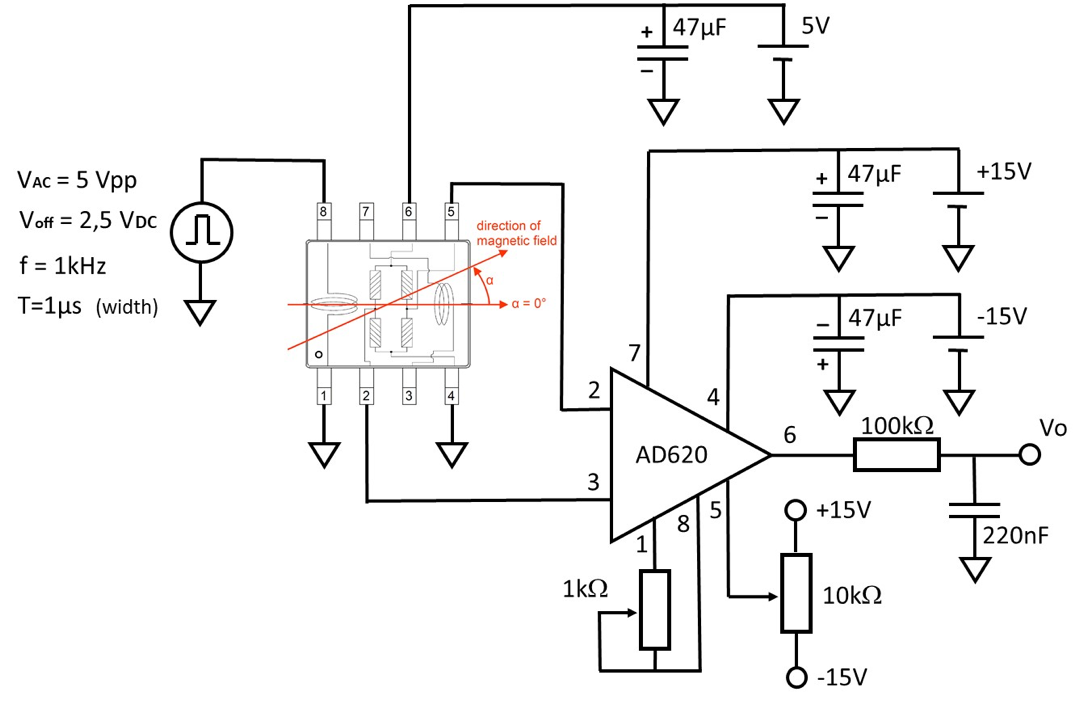
\includegraphics[width=\textwidth]{img/esquema.png}
            \caption{Esquemático.}
        \end{subfigure}
        \begin{subfigure}{0.47\textwidth}
            \centering
            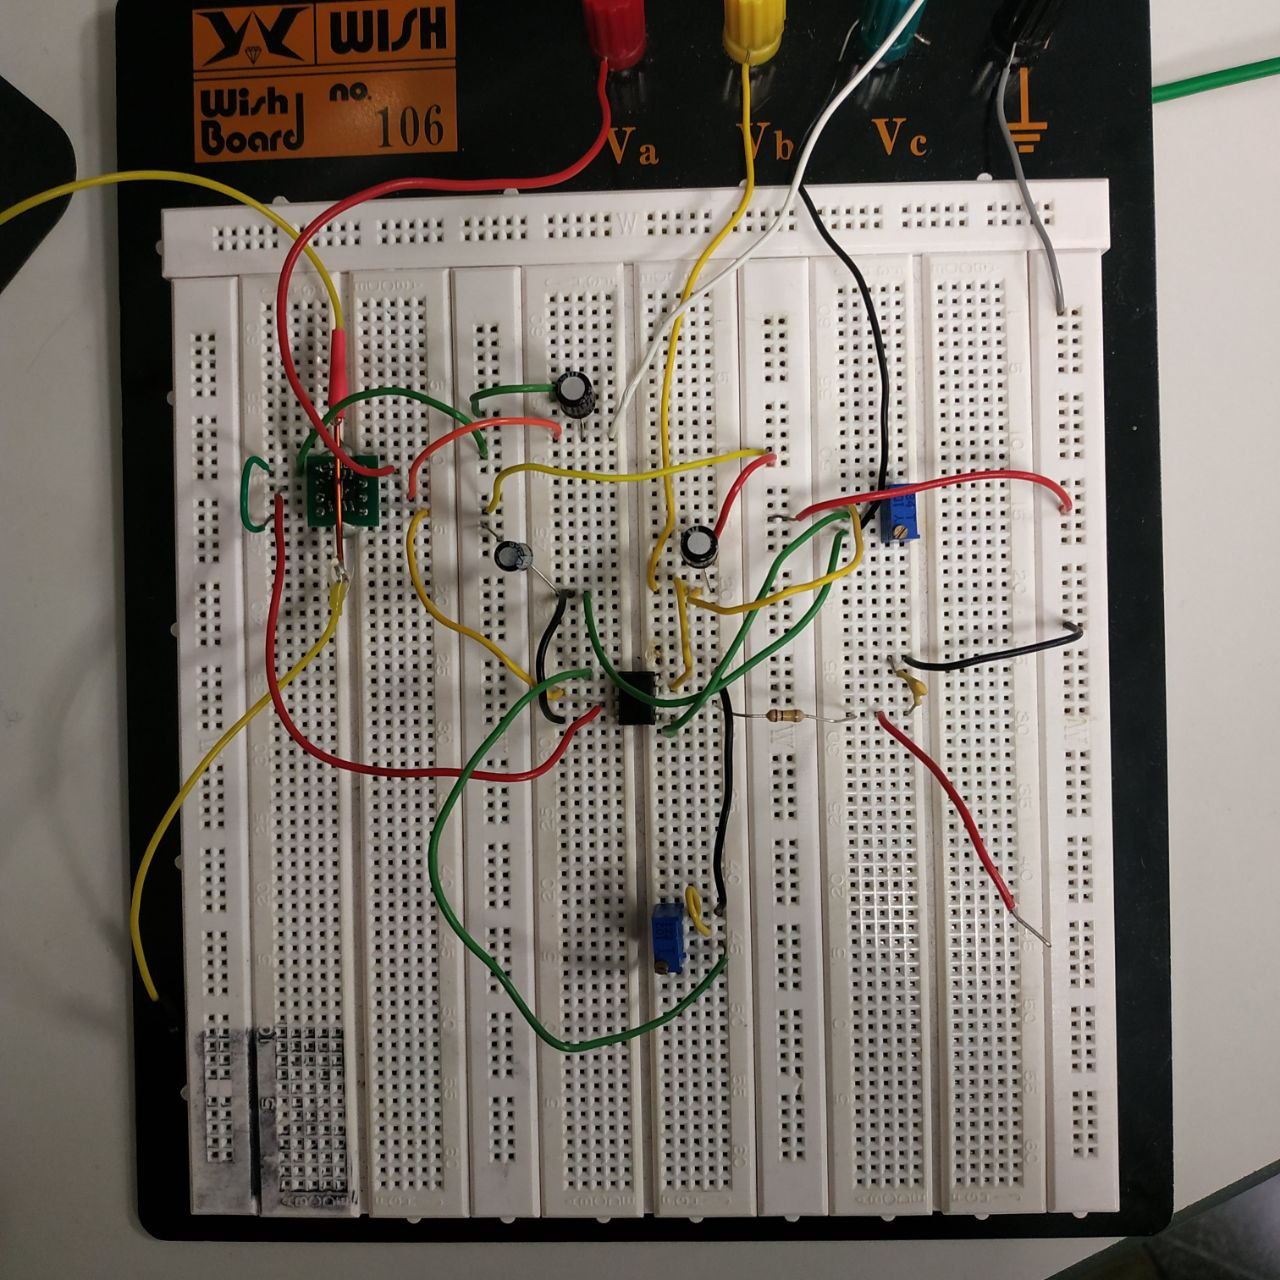
\includegraphics[width=\textwidth]{img/circuito.jpg}
            \caption{Circuito implementado.}
        \end{subfigure}
        \caption{Montaje del circuito.}
        \label{figura}
    \end{figure}
    \item \textbf{Visualización en el osciloscopio de la señal configurada en el generador de funciones antes y después de conectar dicha señal al circuito.} \\
    Aquí se debería hablar de por qué cambian los transitorios al conectarse al circuito...\todo{Hablar de esto e incluir las fotos}
%    \begin{figure}[htb]
%        \centering
%        \begin{subfigure}{0.48\textwidth}
%            \centering
%            \includegraphics[width=\textwidth]{img/pulso_antes.png}
%            \caption{Antes de conectarse al circuito}
%        \end{subfigure}
%        \begin{subfigure}{0.48\textwidth}
%            \centering
%            \includegraphics[width=\textwidth]{img/pulso_despues.jpg}
%            \caption{Tras conectarse al circuito}
%        \end{subfigure}
%        \caption{Pulso configurado en el generador de ondas}
%    \end{figure}
    \item \textbf{Utilizando la fuente variable de tensión como fuente de corriente, se aplica una corriente de 1A al sensor de corriente (hilo de Cu de 1mm de diámetro). Hecho esto, se ajustan los potenciómetros de offset ($10k\Omega$) y de ganancia ($1k\Omega$) para obtener 1V a 1A y tensión nula a corriente nula.}
    \item \textbf{Visualización de la señal DC de salida del acondicionador en el osciloscopio.} \\
    \todo{Incluir las fotos}
%    \begin{figure}[htb]
%        \centering
%        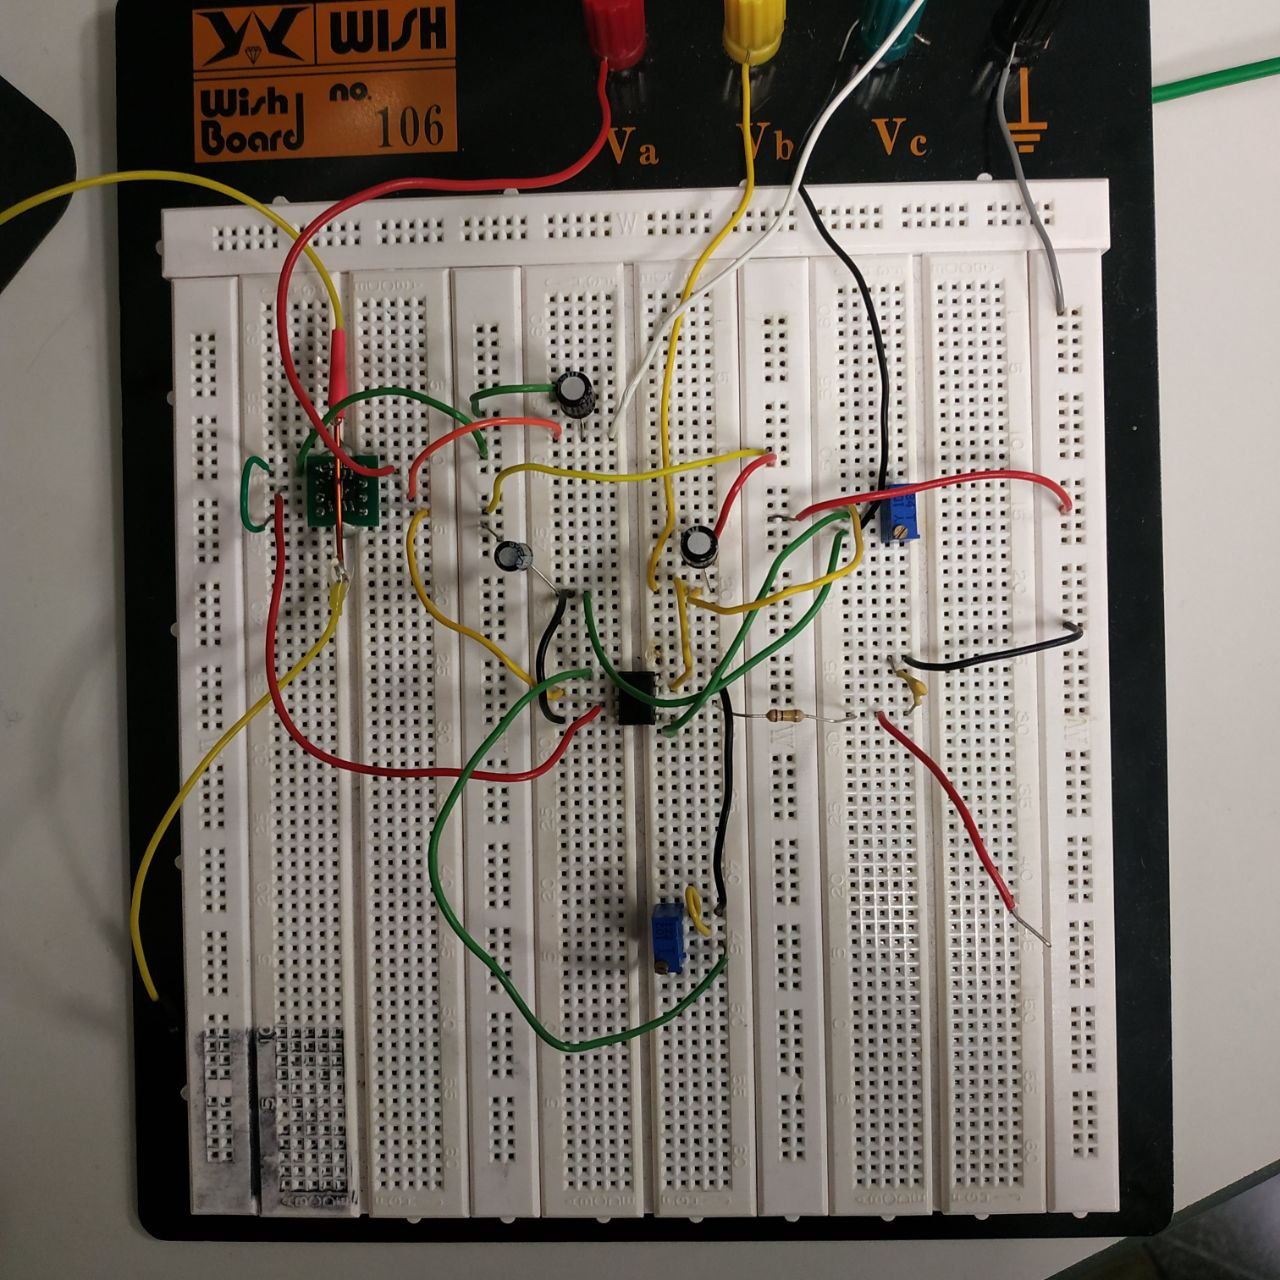
\includegraphics[width=\textwidth]{img/circuito.jpg}
%        \caption{Señal a la salida del circuito.}
%    \end{figure}
\end{enumerate}

\subsection{Caracterización del sensor}

Una vez el amperímetro está implementado y ajustado, se procede a verificar su correcto funcionamiento con lo siguientes procedimientos:

\begin{enumerate}
    \item \textbf{En la siguiente tabla se recogen las tensiones medidas ante determinadas intensidades de corriente.} \\
    Tabla\todo{Tabla}
    \item \textbf{A continuación se representan gráficamente los valores recogidos en la tabla anterior.} \\
    Gráficas y comparación con las gráficas de la ficha técnica.\todo{}
    \item \textbf{Comprobación del efecto del campo terrestre.} \\
    Con el acondicionador ya ajustado tanto en offset como en ganancia de 1V/A, se pueden observar cambios muy significativos en las tensiones medidas al moverlo. Realizando rotaciones de 30º aproximadamente en varios sentidos, se han observado las siguientes variaciones:
    \begin{itemize}
        \item Inclinado hacia los laterales se han producido variaciones de $±100mV$.
        \item Inclinado hacia el frente se han producido variaciones de $±10mV$.
        \item Rotándolo sobre la mesa se han producido variaciones de $±180mV$.
    \end{itemize}
\end{enumerate}
